\subsubsection{Impact of Low-Quality Solutions}
\label{sec:impact-of-noise}
\begin{table*}[!ht]
    \centering
    \caption{SFT performance on the MATH validation set with various filtering strategies to remove solutions with incorrect reasoning.}
    \label{tab:nosiy-data-sft-performance}
    \begin{tabular}{lcc}
    \toprule
     Filtering Strategy    &  Data Size & MATH Validation Accuracy \\ \midrule
     Unfiltered      & 128K &  43.6 $\pm$  1.7 \\
     LLM-as-a-Judge: Prompt 1 & 113K           &  43.6 $\pm$ 0.1 \\ 
     LLM-as-a-Judge: Prompt 2  & 116K          &  43.0 $\pm$
     0.8  
     \\
     Nemotron-4-340B-Reward: Helpfulness $\ge 3$             &  118K &  43.8 $\pm$ 0.4 \\
     Nemotron-4-340B-Reward: Correctness $\ge 3$  &  120K &  43.1 $\pm$ 0.4 
     \\  \bottomrule
    \end{tabular}
\end{table*}



Data quality plays an important role in the accuracy of LLMs~\citep{jain2024llmassisted}.  
We explore the impact of data quality on the final SFT performance in our setup. 
First, we employ automated LLM-based methods to filter out solutions that, despite reaching the correct answer, use incorrect reasoning. Second, we investigate the effects of intentionally incorporating incorrect solutions into the SFT dataset.


\paragraph{Removing Low-Quality Solutions.}
Synthetic solutions produced in our pipeline may include examples where the intermediate steps are incorrect, yet still lead to the right final answer.
For simplicity, we refer to these instances as ``low-quality'' data.  In this section, we will discuss how we identify and remove low-quality data, followed by an investigation into its impact on the SFT performance.

We employ two methods to identify low-quality data: LLM-as-a-Judge and reward model. In the LLM-as-a-Judge approach, we design two  prompts for the \texttt{Llama3.1-405B-Instruct} to determine whether the generated solutions contain incorrect intermediate steps, providing a binary outcome (see Appendix \ref{sec:LLM-as-a-judge-prompt} for the prompts). For the reward model labeling method, we use Nemotron-4-340B-Reward \citep{wang2024helpsteer2} to evaluate the quality of the generated solutions based on factors like helpfulness (the overall usefulness of the response to the prompt) and correctness (the inclusion of all relevant facts without errors). Helpfulness and correctness are rated on a scale from 0 to 4, where a higher score indicates better data quality. For the reward model filtering, we used a threshold of 3 based on small-scale tuning experiments. 

To determine the impact of filtering low-quality data on the SFT performance, we use a 128K-sized fair downsampled SFT dataset. 
We call this \emph{Unfiltered} data and use a model trained on it as a baseline. 


Table \ref{tab:nosiy-data-sft-performance} presents the statistics of data remaining with different filtering approaches, and the corresponding SFT performance. 
The proportion of data filtered by the different methods ranges from 6\% to 12\%, a non-negligible fraction of the overall data. \footnote{Our manual analysis of 20 examples identified by the two approaches suggests that approximately 60\% of the solutions are indeed incorrect.}
Yet none of the filtering strategies give any meaningful gain over the baseline \emph{Unfiltered} model. 
This means that either SFT is robust to the presence of up to 10\% of low-quality solutions or our filtering is not accurate enough. We investigate this question next.


\begin{figure*}[ht]
    \centering
    \begin{subfigure}[b]{0.45\textwidth}
        \captionsetup{justification=centering}
        \centering
        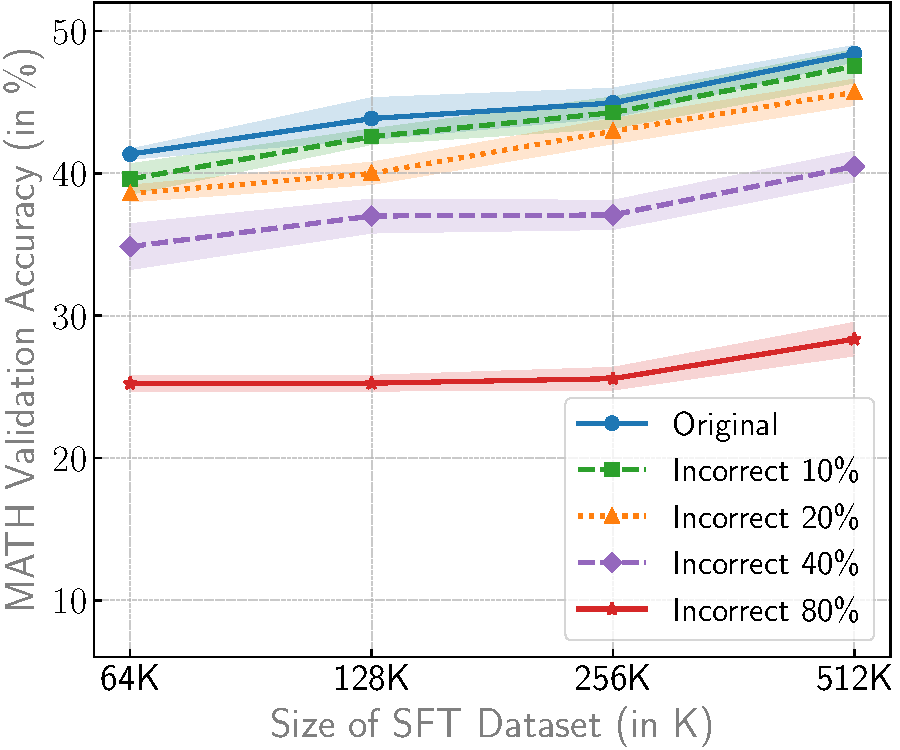
\includegraphics[width=\textwidth]{plots/noise_solution_with_err_bar.pdf}  %
        \caption{Adding wrong-answer solutions.}
        \label{fig:figure1}
    \end{subfigure}
    \hfill
    \begin{subfigure}[b]{0.45\textwidth}
    \captionsetup{justification=centering}
        \centering
        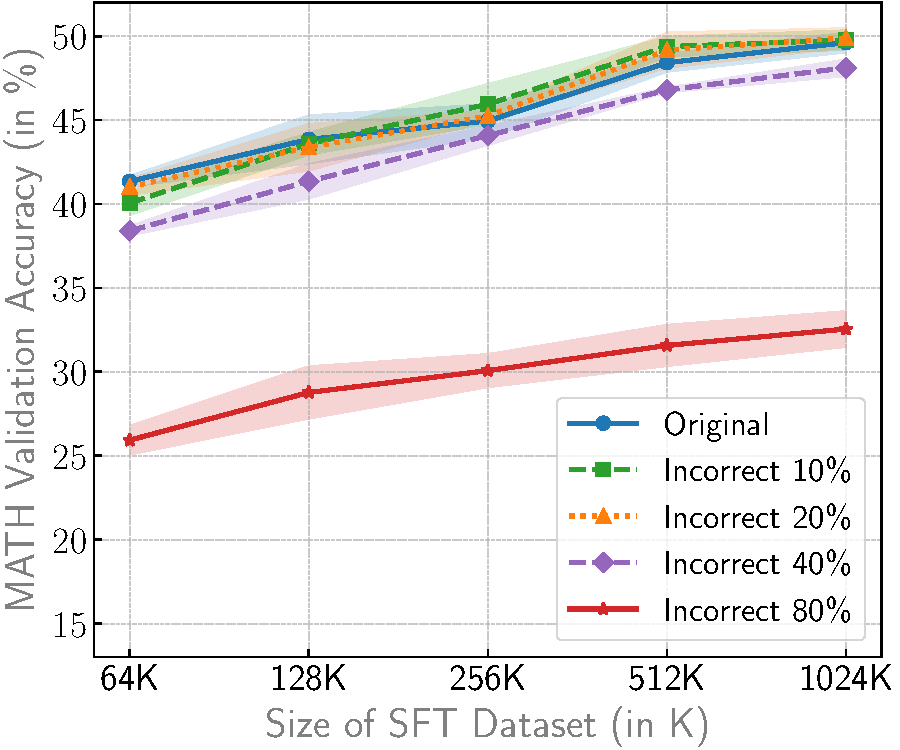
\includegraphics[width=\textwidth]{plots/noise_pairing_with_err_bar.pdf}  %
        \caption{Correct solutions mismatched with questions}
        \label{fig:figure2}
    \end{subfigure}
    
    \captionsetup{justification=centering}\caption{Impact of low-quality solutions on the SFT performance. }
    % \vspace{-0.2in}
    \label{fig:incorrect_solutions}
\end{figure*}









\paragraph{Adding Low-Quality Solutions.}


In the previous section, we see that filtering low-quality solutions generated by a strong model such as \texttt{Llama3.1-405B-Instruct} leads to almost the same or worse SFT performance in comparison to no filtering. 
While our manual analysis suggests that most of the filtered out solutions were indeed using incorrect reasoning, the automatic filtering approaches are far from perfect and it's hard to gauge the impact of filtering out correct solutions which have been classified as incorrect. 

To remove the effect of potentially inaccurate filtering, we can instead study the impact of explicitly adding low-quality/incorrect solutions on the SFT performance. 
We consider two strategies of adding ``bad'' solutions:
\begin{enumerate}
    \item \textbf{Wrong-answer Solutions}: By incorporating solutions generated by the teacher LLM, which were excluded during the creation of the SFT dataset due to not arriving at the ground truth answer.
    \item \textbf{Incorrect Pairing}: 
    By shuffling some of the question-solution pairs in the SFT dataset, such that the correct solutions are paired with unrelated questions.  
\end{enumerate}

For both these strategies, we experiment with varying the proportion of such incorrect solutions from \{10\%, 20\%, 40\%, 80\%\}. 
We also vary the SFT data size from  \{64K, 128K, 256K, 512K, 1024K\} to study the impact on SFT performance at different data scales\footnote{For the ``Wrong-answer Solutions'' setting, we were not able to run the experiments for 1024K data size because the \texttt{Llama3.1-405B-Instruct} model makes few mistakes on the MATH training set.}.  

Figure~\ref{fig:incorrect_solutions} presents the impact of incorrect solutions on the SFT performance at varying data sizes. 
From both the plots we see that the model performance suffers little to no performance degradation with as much as 20\% incorrect solutions at data scales $\ge 256$K. Among the two strategies, we see that the model is especially robust to ``Incorrect Pairing'' with strong performance even with 40\% incorrect solutions. 

Based on these results we conclude that models are indeed robust to the presence of up-to 20\% of low-quality solutions during SFT and extensive data filtering at this stage has limited gains.
